Uczenie maszynowe, znane również jako machine learning, to specjalistyczna gałąź sztucznej inteligencji,
która koncentruje się na konstruowaniu modeli i algorytmów umożliwiajcych komputerom samodzielne uczenie się z dostępnych danych.
W przeciwieństwie do systemów, które są bezpośrednio programowane do wykonania określonych zadań,
systemy uczenia maszynowego analizują dane, rozpoznają wzorce i podejmują decyzje oparte na zdobytej w ten sposób wiedzy.

\subsection{Definicje}

\noindent
\textbf{Definicja 1.}
Zbiór uczący

\noindent
\textbf{Definicja 2.}
Zbiór walidacjny

\noindent
\textbf{Definicja 3.}
Zbiór testowy

\noindent
\textbf{Definicja 4.}
Walidacja krzyżowa

\noindent
\textbf{Definicja 5.}
Warstwa Rescaling

\noindent
\textbf{Definicja 6.}
Warstwa Conv2D

\noindent
\textbf{Definicja 7.}
Epoka

\noindent
\textbf{Definicja 8.}
Regularyzacja

\noindent
\textbf{Definicja 9.}
Współczynnik dropout

\noindent
\textbf{Definicja 10.}
Dokładność modelu

\noindent
\textbf{Definicja 11.}
Strata modelu

\noindent
\textbf{Definicja 12.}
Przeuczenie

\noindent
\textbf{Definicja 13.}
Algorytm t-SNE

\subsection{Rodzaje uczenia maszynowego}
Według \cite{Geron2020}, uczenie maszynowe można sklasyfikować na podstawie kilku kryteriów.
Jest to nadzór człowieka w procesie trenowania, możliwość modelu do uczenia się w czasie rzeczywistym
oraz sam sposób pracy (nauka z przykładów lub modelu). Kryteria te nie wykluczają się wzajemnie - można je dowolnie łączyć.
Za przykład może posłużyć filtr antyspamowy, który ciągle się uczy,
wykorzystując model sieci neuronowej i analizując wiadomości email.
Taki system można określić przyrostowym, opartym na modelu i nadzorowanym.

Dodatkowe kryteria oceny rodzaju uczenia maszynowego:
\begin{itemize}[label=-,labelsep=0.4cm,leftmargin=0.6cm]
    \item Uczenie nadzorowane (ang. supervised learning) to podejście, w którym model jest szkolony na danych,
        które są już odpowiednio oznaczone (np. rekordy mają przypisane odpowiednie klasy).
        Celem jest odkrycie funkcji, która przekształca dane wejściowe w oczekiwane wyjścia.
        Znajduje zastosowanie w klasyfikacji i regresji.
        Przykład: Klasyfikacja wiadomości e-mail jako spam lub nie-spam.
    \item Uczenie nienadzorowane (ang. unsupervised learning)
        - w tym przypadku model bada nieoznaczone dane, aby odkryć pewne wzorce lub struktury.
        Najczęściej stosowane w klasteryzacji, czy redukcji wymiarowości. Przykłady:
        \begin{itemize}[label=*,labelsep=0.4cm,leftmargin=0.8cm]
            \item Klasteryzacja klientów w celu segmentacji rynku, gdzie klienci są grupowani na podstawie ich zachowań zakupowych. 
            \item Redukcja wymiarowości w celu wizualizacji danych wysokowymiarowych, np. za pomocą algorytmu t-SNE.
        \end{itemize}
    \item Uczenie przez wzmacnianie (ang. reinforcement learning) to przypadek,
        gdzie model uczy się poprzez interakcję ze swoim otoczeniem,
        podejmując decyzje, które maksymalizują pewną nagrodę. Przykłady:
        \begin{itemize}[label=*,labelsep=0.4cm,leftmargin=0.8cm]
            \item Algorytmy sterujące robotami, które uczą się poruszać w nieznanym terenie. 
            \item Programy grające w gry, takie jak AlphaGo (chińska gra Go), które uczą się strategii gry poprzez rozgrywanie wielu partii.
        \end{itemize}
\end{itemize}

\subsection{Proces uczenia maszynowego}
Proces uczenia maszynowego można podzielić na kilka etapów,
które są niezbędne do stworzenia skutecznego modelu zdolnego do samodzielnej nauki na podstawie zebranych danych.

Należy rozpocząć od zgromadzenia danych z odpowiednich źródeł.
Mogą obejmować bazy danych, API, pliki CSV, czujniki, logi systemowe czy nawet wpisy z mediów społecznościowych.
Dane mogą być ustrukturyzowane (np. tabele w bazach danych) lub nieustrukturyzowane (np. obrazy, tekst).

Dalej, konieczne jest przygotowanie danych do odpowiedniego formatu.
Obejmuje to usunięcie brakujących, pustych oraz błędnych wartości,
radzenie sobie z duplikatami i anomaliami, skalowanie cech, kodowanie zmiennych kategorycznych,
normalizację danych oraz podzielenie danych na zbiory treningowe, walidacyjne i testowe.

\begin{figure}[ht]
	\centering
	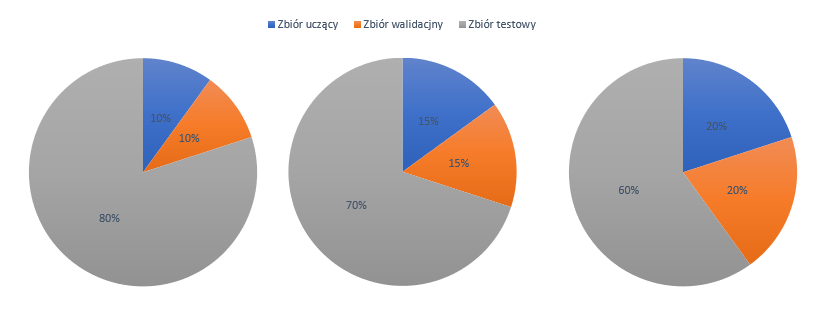
\includegraphics[height=11cm]{partials/images/machine_learning_process_1.png} % do zmiany
	\caption{Przykład podziału danych na zbiory treningowe, walidacyjne i testowe}
\label{Fig:MachineLearningProcess1}
\end{figure}

Najczęściej, podział na zbiory dokonuje się w proporcjach 70-80\% na trening, 10-15\% na walidację i 10-15\% na testy.
Jest to zależne od specyfiki problemu,
dlatego konieczne jest odpowiednie przygotowanie i zbadanie danych przed podjęciem decyzji.

Wybór modelu to proces, który zależy od rodzaju problemu (np. regresja, klasyfikacja, klasteryzacja)
oraz charakterystyki danych, gdzie najpopularniejsze modele to drzewa decyzyjne,
lasy losowe, maszyny wektorów nośnych (SVM), sieci neuronowe, k-najbliższych sąsiadów (k-NN)
i regresja liniowa/logistyczna. Trenowanie modelu to kolejny etap,
który polega na dostosowaniu parametrów modelu do danych treningowych,
w tym dostosowaniu hyperparametrów modelu (parametrów, które nie są uczone,
np. liczba warstw w sieci neuronowej) poprzez metodę walidacji krzyżowej lub inne techniki optymalizacji.

Ewaluacja obejmuje ocenę modelu za pomocą pewnych metryk,
takich jak dokładność, precyzja, recall, F1-score, błąd średniokwadratowy (MSE),
błąd absolutny (MAE), a także analizy wydajności modelu w przypadku klasyfikacji binarnej.
Optymalizacja modelu to kolejny etap, który obejmuje dalsze dostosowanie hyperparametrów,
wybór cech, które najbardziej wpływają na wynik modelu,
próby różnych architektur modelu oraz zastosowanie technik takich jak L1, L2, dropout,
które zapobiegają przeuczeniu modelu.

Implementacja modelu jest procesem, w którym wdrażany jest model w środowisku produkcyjnym.
Zakłada ona przeprowadzenie integracji z aplikacjami zewnętrznymi, tworzenie API serwujących dane,
zautomatyzoawanie decyzji, czy też śledzenie wydajności modelu w czasie rzeczywistym,
aby wykryć ewentualne pogorszenie jakości (drift danych) i regularne aktualizacje modelu.
Aktualizacja i utrzymanie modelu to kolejny etap,
który obejmuje regularne aktualizowanie modelu na podstawie nowych danych,
aby utrzymać jego dokładność i skuteczność, ciągłe monitorowanie,
aby zapewnić, że model działa zgodnie z oczekiwaniami i nie występują niepożądane zachowania.
Proces uczenia maszynowego jest iteracyjny i wymaga ciągłej interakcji między danymi,
modelem i wynikami, aby osiągnąć optymalne rezultaty.